\Chapter{Implementáció}

A fejezet a program készítése során felmerülő problémák leírásával foglalkozik. Bemutatja hogyan sikerült az alkalmazás egyes részeit implementálnom. Nem tartalmaz a program használatával kapcsolatos információkat. 
\\A fejezet felépítése a program csomag-szintű felépítésével egyezik.

\Section{Data}

Az előző fejezetben leírt szükséges adattípusokat egy \texttt{Content} nevű osztályba gyűjtöttem össze. A csomag felépítése \aref{fig:package_data}. ábrán látható.
\vspace{5pt}\\Két tároló objektumot tartalmaz, amelyek \texttt{DefaultListModel} típusúak, ezen belül \texttt{Note} és \texttt{Page} típusú adatokat tartalmaznak. \texttt{DefaultListModel} objektumot egy lista elemeinek létrehozására és megjelenítésére használjuk Java-ban. Mivel az adatok csak listákban kerülnek megjelenítésre, ezért ez az objektum tökéletes volt az adatok tárolására.
\vspace{5pt}\\Az alkalmazás azon részei, amelyek az adatokkal dolgoznak a \texttt{Content} osztályon keresztül érik el őket.
\begin{figure}[h]
	\centering
	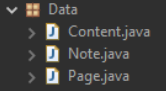
\includegraphics[scale=0.7]{images/package_data.png}
	\caption{Data csomag és osztályai}
	\label{fig:package_data}
\end{figure}

\Section{Database}
Egy osztályt tartalmaz, a \texttt{DatabaseFunctions}-t, amiben az adatbázissal kapcsolatos funkciókat gyűjtöttem össze, mint az adatbázishoz való csatlakozás, fájlok fel- és letöltése. A csomag felépítése a \ref{fig:package_database}. ábrán látható.
\vspace{5pt}\\Az adatok Firebase nevű felhőalapú adatbázisban kerülnek tárolásra, így az alkalmazás megfelelő működéséhez szükséges van internetkapcsolatra.
\\Az alkalmazást át kellett alakítanom Maven project-re, hogy a Firebase adatbázis driver-éhez hozzá tudjak férni, majd az API segítségével kapcsolatba tudjak lépni az adatbázissal.
\\Lehetsőségünk van Firebase-en belül \texttt{Blob (Binary large object/Nagy bináris objektum)} fájlok tárolására. Az alkalmazás adatai titkosított XML fájl formájában kerülnek az adatbázisba. A Firebase ezen felül data-at-rest titkosítást is alkalmaz.
\begin{figure}[h]
	\centering
	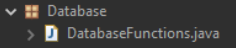
\includegraphics[scale=0.7]{images/package_database.png}
	\caption{Database csomag és osztálya}
	\label{fig:package_database}
\end{figure}

\Section{Encryption}
Titkosítással kapcsolatos osztályokat tartalmaz. A csomag felépítése a \ref{fig:package_encryption}. ábrán látható.
\vspace{5pt}\\Az \texttt{AppKeyStore} osztálynak két funkciója van. 
\\Egyik egy random generált 256 bit-es AES titkosítási kulcs létrehozására szolgál, amit egy \texttt{KeyStore} objektumban tárol, ezt .jks kiterjesztésű 256 karakter hosszú jelszóval védett fájlként tárolja. A fájl a program működése alatt feltöltődik az adatbázisba.
\\A jelszó karakterek random sorozatából áll, de minden .jks fájl ugyanazzal a jelszóval van védve. Vitatható, hogy ez a megoldás biztonságos-e, úgy gondolom, hogy igen, a jelszó hosszából és karaktereiből ítélve, ugyanis nem csak számokat és betűket tartalmaz, hanem szimbólumokat is.
\\Adatbázisba töltését szükségszerűnek tartom, hogy különböző eszközökön is el tudjuk érni ugyanazt a tartalmat.
\\Másik metódusa segítségével letölti az adatbázisból a .jks fájlt, amit ideiglenesen eltárol az eszközön, majd ebből az ideiglenes fájlból éri el a korábban létrehozott titkosítási kulcsot.
\vspace{5pt}\\Az \texttt{EncryptionFunctions} osztály a titkosítást és visszafejtést végző funkciókat tartalmazza. Ezek a műveletek a .jks fájlba elmentett random generált kulcsot alkalmazzák az XML fájl titkosításához és visszafejtéséhez.
\\A funkciók AES algoritmust használnak, működésük megegyezik az algoritmusok összehasonlításához használt tesztalkalmazás működésével, a \texttt{javax.crypto} csomag osztályait alkalmaztam.

\begin{figure}[h]
	\centering
	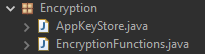
\includegraphics[scale=0.7]{images/package_encryption.png}
	\caption{Encryption csomag és osztályai}
	\label{fig:package_encryption}
\end{figure}

\Section{XML}
A csomag XML-lel foglalkozó osztályokat tartalmaz, felépítése a \ref{fig:package_xml}. ábrán látható. Ilyen az \texttt{XMLReader}, ami olvassa és parzolja az adott XML fájlt. Az \texttt{XMLWriter} XML dokumentum írását és formázását végzi.
\vspace{5pt}\\A program a szükséges fájlokat egy \texttt{config.xml}-nek nevezett dokumentumból éri el, aminek írását és olvasását a \texttt{ConfigManager} osztály végzi. Ennek az osztálynak a részletes működését a következő fejezet tartalmazza.


\begin{figure}[h]
	\centering
	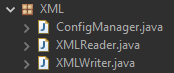
\includegraphics[scale=0.7]{images/package_xml.png}
	\caption{XML csomag és osztályai}
	\label{fig:package_xml}
\end{figure}

\Section{GUI}
Ez a csomag a felhasználói felület főbb osztályait tartalmazza (lásd \ref{fig:package_gui}. ábra).
\vspace{5pt}\\Legnehezebb dolgom a \texttt{TextEditorButtons} nevű osztállyal volt, ami a 4.1.3-mas alfejezetben leírt szövegszerkesztő megfelelő működését biztosítja. A felhasználói felület készítése során ennek az osztálynak létrehozása volt a legidőigényesebb feladat.
\\Alapértelmezett beállítás a 12-es nagyság, fehér szín és Dialog betűstílus. A szövegszerkesztőbe beírt adatok és a szövegszerkesztő gombjai között nincs valós-idejű kapcsolat.
\\Ezt egy példával tudom legjobban elmagyarázni: ha a szöveg egy részének (a gombok ugye csak a kijelölt részeket szerkesztik) stílusát megváltoztatjuk, tegyük fel 18-as betűméret, piros szín és Times New Roman betűstílusra, a gombokon feltüntetett szöveg megváltozik. Ha a kurzorral egy nem szerkesztett szövegrészre kattintunk, akkor a gombok állapota nem áll vissza az alapértelmezett beállításokra, hanem az utoljára beállított opción marad (tehát nem lesz Dialog-12-fehér, hanem Times New Roman-18-piros marad).


\begin{figure}[h]
	\centering
	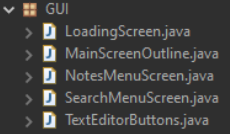
\includegraphics[scale=0.7]{images/package_gui.png}
	\caption{GUI csomag és osztályai}
	\label{fig:package_gui}
\end{figure}


\Section{GUIRelated}
A csomag olyan osztályokat tartalmaz, amelyek a grafikus felhasználói felület személyre szabásában segítettek. A csomag felépítése a \ref{fig:package_guirelated}. ábrán látható.
\begin{figure}[h]
	\centering
	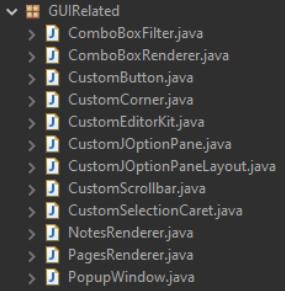
\includegraphics[scale=0.6]{images/package_guirelated.png}
	\caption{GUIRelated csomag és osztályai}
	\label{fig:package_guirelated}
\end{figure}
\\A felhasználói felületet \texttt{Java Swing} használatával készítettem. Ahhoz, hogy megértsük milyen nehézségekkel szembesültem, egy rövid leírásban be kell mutassam a függvénykönyvtárat:
\vspace{10pt}\\A Swing egy GUI widget toolkit. Widget-ek alatt olyan grafikus elemeket értünk, mint gombok, szövegdobozok, listák, legördülő menük, görgők, stb...
\\A Swing egy régi technológia, viszont rengeteg alkalmazás használja. A Java GUI készítésre létrehoztak egy modernebb függvénykönyvtárat, ami a Swing-re épül, a \texttt{JavaFX}-et.
\\Kevésbé használt, mint a Swing, valószínűleg azért, mivel az alkalmazások nagy része korábban, Swing-ben készült, és nincs szükség JavaFX-szé való konvertálásukra. Új Java GUI-k készítésére valószínűnek tartom, hogy inkább JavaFX-et használnak.
\vspace{10pt}\\Azért választottam a Swing-et a JavaFX helyett, mert már dolgoztam a könyvtárral, míg a JavaFX-et egyáltalán nem ismertem, így azt gondoltam, hogy egyszerűbb dolgom lesz.
\\Hamar rá kellett jönnöm, hogy nem lesz olyan egyszerű dolgom, mint amire számítottam, de ettől függetlenül maradtam a Swing használata mellett. Ahhoz, hogy a widget-eknek egy modern megjelenést tudjunk adni, rengeteg szülőosztály-beli metódust kell megvizsgálnunk és felülírnunk. Sok esetben nem érhető el olyan funkció, amit logikusnak tartanánk, hogy létezik és közvetlenül szerkeszthető. Pár példa, hogy mire is gondolok:
\vspace{5pt}\\A \texttt{JButton} widget egy gomb, amire lehet szöveget írni. Ha megnyomjuk a gombot, megváltozik a háttérszíne, amíg el nem engedjük az egérgombot. Ezt a színt közvetlenül egy metódussal nem lehet megváltoztatni. A felülírt kódról egy részlet a \ref{fig:package_guirelated_jbutton}. ábrán látható
\begin{figure}[h]
	\centering
	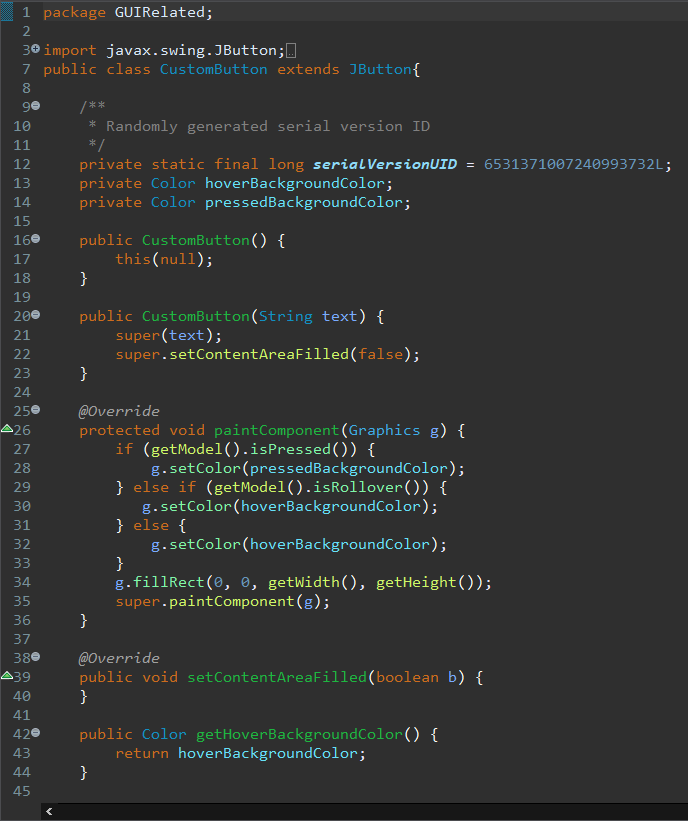
\includegraphics[scale=0.3]{images/package_guirelated_jbutton_details.png}
	\caption{JButton megjelenését felülírő osztály}
	\label{fig:package_guirelated_jbutton}
\end{figure}
\\A \texttt{JList} listaelemek háttérszínét, legyen-e az elemeknek kerete vagy sem, elemek szövegének színét sem lehet közvetlen metódussal megváltoztatni. A felülírt kódról egy részlet a \ref{fig:package_guirelated_jlistrenderer}. ábrán látható
\begin{figure}[h]
	\centering
	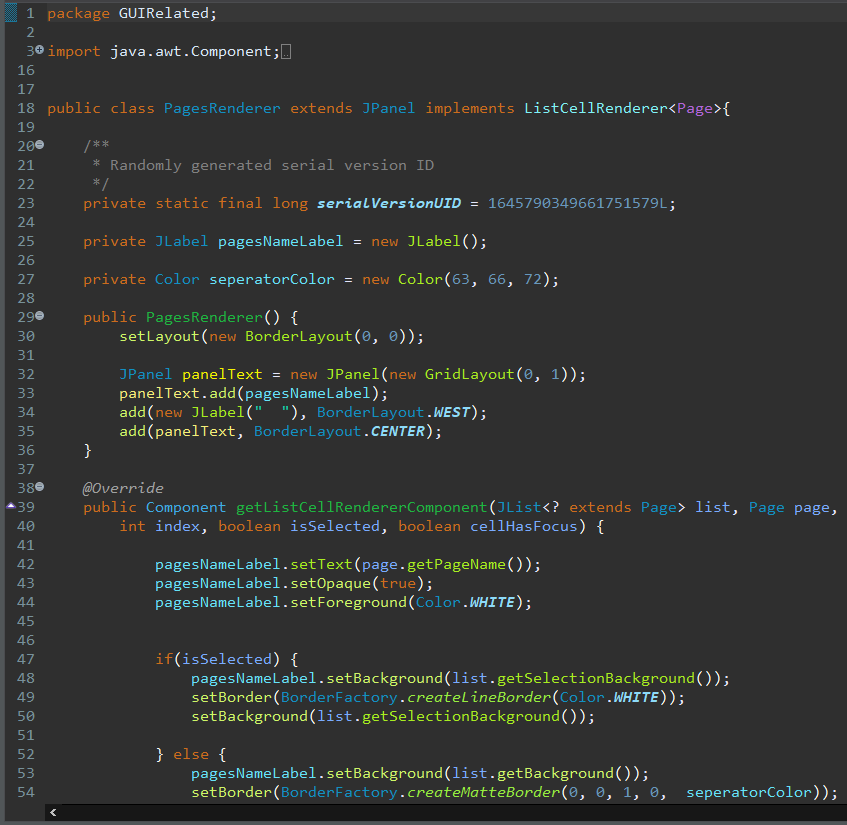
\includegraphics[scale=0.3]{images/package_guirelated_jlistrenderer_details.png}
	\caption{JList listaelemeit renderelő osztály}
	\label{fig:package_guirelated_jlistrenderer}
\end{figure}
\vspace{5pt} \\ \noindent A csomag összes osztálya ilyen jellegű problémákat old meg, szükségesek az elképzelt, modern felhasználói felület létrehozásához.


\Section{Main}
A csomag a fő futtatható osztályt tartalmazza. Internetkapcsolat ellenőrző függvényt és az alkalmazás adatait betöltő algoritmusokat tartalmazza. A csomag felépítése a \ref{fig:package_main}. ábrán látható.

\begin{figure}[h]
	\centering
	
\includegraphics[scale=0.6]{images/package_main.png}
	\caption{Main csomag és osztálya}
	\label{fig:package_main}
\end{figure}


\Section{További fejlesztési lehetőségek}
Egyik opció sem kulcsfontosságú az alkalmazás működésének szempontjából, azért nem kerültek bele a program végső verziójába. Hasznos funkciók, de némelyik inkább csak a kényelmet szolgálja.
\\Az ötletek nagy részének későbbi megvalósítása ettől függetlenül tervbe van.

\subsection{Automatikus elindulás}
A program automatikusan induljon el az eszköz indításakor.

\subsection{Naptár és emlékeztető}
Az első megvalósítandó ötlet egy naptár elhelyezése az alkalmazás kettő meglévő menüje mellé.
\\Ez a képernyő jelenne meg alkalmazás indulásakor, főmenü szerepet töltene be.
\vspace{5pt}\\A felületen lenne egy naptár, amit lehetne időben előre-hátra lapozni, akárcsak egy rendes naptárat.
\vspace{5pt}\\Emlékeztető írására alkalmas funkciókat is kéne tartalmazzon, ez lenne a menüpont lényege. A felhasználó írhatna egy emlékeztetőt egy jövőbeli eseményre (múltbeli eseményre hibát dobna) és be lehetne állítani, hogy mikor emlékeztessen (aznap, egy nappal előtte, két nappal előtte, stb..).
\vspace{5pt}\\Emlékeztető alatt egy felugró ablakra gondolok, ami attól függetlenül, hogy milyen ablakok vannak még megnyitva (legyen az böngésző, vagy másik alkalmazás), azok felett lenne (on top). 
\\Felépítése hasonló lenne a jegyzet/lap törlése modális ablakéhoz.
Tartalmazna egy 'OK' gombot, ami bezárja ezt az ablakot, és egy 'Remind me later' gombot, ami ideiglenesen bezárja az ablakot, majd X perc múlva ismét megjeleníti. A gombok felett jelenne meg az emlékeztető szövege.


\subsection{Beállítások}
Egy felugró ablak, tele opciókkal.
\\Kimondottan a felhasználói felület megváltoztatására alkalmas beállításokra gondolok (pl.: színek variálása), de akár működés	módosítására alkalmas beállításokat is tartalmazhatna ez az ablak.
\\Két titkosítási opciót is el lehetne itt helyezni. Ezalatt arra gondolok, hogy alkalmazás szintű titkosítási megoldást alkalmazzon az applikáció vagy elegendőnek tartja a felhasználó az adatbázis at-rest titkosítását, amit a szolgáltató végez.

